\chapter{ترنسفورمر ها و تاریخچه آنها}

از آنجایی که ریشه معماری ترنسفورمر در ترجمه ماشینی و شبکه های عصبی بازگشتی است و معماری های پردازش تصویر بر پایه ترنسفورمر هم به‌شدت از این مفاهیم استفاده می‌کنند، لازم است تا مقدماتی را توضیح دهیم. در این فصل به بررسی RNN ها، شبکه های کاهشی-افزایشی، مکانیزم توجه، معماری ترنسفورمر در حالت خاص ترجمه ماشینی، و در نهایت اقتباس آن‌ها برای عملیات‌های پردازش تصویر می‌پردازیم.

\section{ ترجمه ماشینی}
مسئله ترجمه ماشینی به این صورت تعریف می‌شود که دنباله‌ای از ورودی‌ها $X = \{x_1, x_2, \dots, x_N\}$ در زبان مبدأ داده شده و هدف پیش‌بینی دنباله خروجی $Y = \{y_1, y_2, \dots, y_T\}$ در زبان مقصد است. در اینجا $x_N$ و $ y_T $ به ترتیب به عنوان نشانگر پایان جمله (\texttt{</s>}) در نظر گرفته می‌شوند و $ y_0 $
برابر با شروع جمله (\texttt{<s>}) است. مدل یادگیری ماشین در تلاش برای یافتن عبارت زیر است.

\begin{equation}
\hat{Y} = \arg\max_{Y} P_\theta(Y | X)
\end{equation}

\section{ ترجمه ماشینی بازگشتی}



برای گسترش این فرمول، از قضیه زنجیره‌ای استفاده می‌کنیم تا احتمال شرطی $P_\theta(Y|X)$ را به حاصل‌ضرب احتمالات شرطی تقسیم کنیم:

\begin{align}
	P_{\theta }(Y \mid X) & = P_{\theta }(y_{1:T} \mid X)  \notag \\
	& = P_{\theta }(y_{T} \mid y_{1:T-1}, X) 
	P_{\theta }(y_{T-1} \mid y_{1:T-2}, X)
	...
	P_{\theta }(y_{1} \mid X) \notag \\
	& = \prod_{t=1}^{T} P_\theta(y_t | y_{1:t-1}, X)
\end{align}

فرآیند به این صورت است که مدل، با داشتن ورودی $X$ و دنباله تولید شده تا زمان $t-1$ یعنی $y_{1:t-1}$، احتمال $y_t$ را پیش‌بینی می‌کند. ایده اصلی در مدل‌های ترجمه ماشینی این است که فرایند تولید خروجی $Y$ به صورت ترتیبی انجام می‌شود و در هر مرحله، مدل به خروجی‌های قبلی وابسته است.  برای مدل‌سازی این فرآیند، دو بخش اصلی وجود دارد: کدگذار \lr{(Encoder)} و رمزگشا \lr{(Decoder)}.
\section{شبکه های کدگذار-رمزگشا (افزایشی-کاهشی)\protect\LTRfootnote{Encoder-Decoder Networks}}
شبکه‌های کدگذار-رمزگشا یکی از معماری‌های متداول در یادگیری عمیق هستند که به‌طور خاص برای مسائل نیاز1

\subsection{کدگذار (Encoder)}

کدگذار وظیفه دارد اطلاعات توالی ورودی را به یک بازنمایی فشرده تبدیل کند. این فرآیند با استفاده از یک تابع بازگشتی به شکل زیر انجام می‌شود:

$$
h_n = f(x_n, h_{n-1})
$$

که در آن $h_{n-1}$ وضعیت نهان در زمان $ n-1 $ است و $x_n$ ورودی فعلی رمزگذار است.

در نهایت، یک نمایش زمینه‌ای $ c $ با ترکیب بازگشتی بردارهای مخفی $ h $ تولید می‌شود:

$$
c = q(h_{1:N}) = h_N
$$

\subsection{کدگشا (Decoder)}
کدگشا از نمایندگی فشرده تولیدشده توسط کدگذار استفاده کرده و آن را به خروجی مورد نظر نگاشت می‌دهد. این بخش نیز معمولاً از همان نوع شبکه‌های کدگذار استفاده می‌کند، اما با هدف تولید خروجی. فرآیند رمزگشا می‌تواند به شکل مرحله‌به‌مرحله باشد، به‌طوری که هر خروجی تولیدشده به‌عنوان ورودی برای مرحله بعدی استفاده می‌شود.
$$
s_t = g(y_{t-1}, c, s_{t-1})
$$

در اینجا $ g $ تابع تغییر حالت است، $ y_{t-1} $ جاسازی%
\LTRfootnote{Embedding}
آخرین خروجی تخمینی کدگشا است، $s_{t-1}$ آخرین وضعیت نهان کدگشا و $c$ نمایندگی فشرده تولیدشده توسط کدگذار است که یک بازنمایی از کل دنباله ورودی را در بر دارد.

معمولا هر وضعیت نهان $s_t$ به یک عملیات خروجی داده می شود تا در نهایت بدست آید:
$$ P_{\theta}(y_{t} | y_{1:t-1},c) $$

\begin{figure}
	\centering
	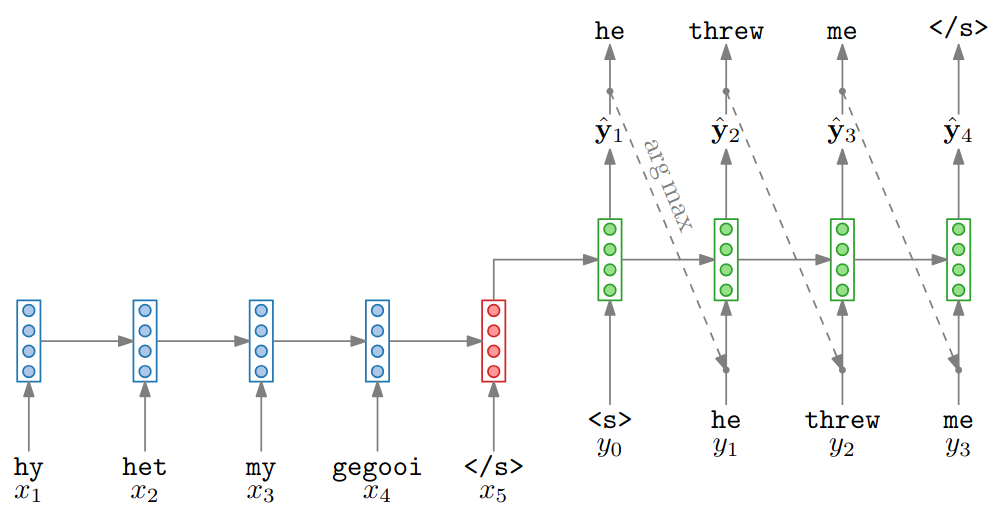
\includegraphics[width=1\linewidth]{figs/rnn_without_attn}
	\caption{نمای کلی یک مدل ترجمه ماشینی بر پایه خروجی های بازگشتی. هدف این شبکه آن است که بازنمایی فشرده و خلاصه ای از کل جمله را در آخرین نشانه ورودی
	($\mathbf{</s>}$)
	جای دهد و کدگشا با تکیه بر همین بردار نهایی، به‌صورت بازگشتی خروجی ترجمه شده را تولید کند.
	}
	\label{fig:rnnwithoutattn}
\end{figure}


یکی از محدودیت‌های اصلی معماری کدگذار-رمزگشا \lr{(Encoder-Decoder) } در مدیریت توالی‌های بلند، وابستگی بیش از حد آن به بردار زمینه \lr{(Context Vector)} است. در این معماری، کدگذار ورودی را به یک بردار فشرده واحد تبدیل می‌کند که حاوی اطلاعات معنایی کل توالی است. سپس رمزگشا از این بردار به‌عنوان منبع اصلی اطلاعات برای تولید خروجی استفاده می‌کند. با افزایش طول توالی ورودی، نمایندگی این بردار فشرده ناکارآمد می‌شود و اطلاعات مهم در فرآیند فشرده‌سازی از بین می‌رود. این محدودیت به‌ویژه در مسائلی مانند ترجمه ماشینی، جایی که وابستگی‌های معنایی میان کلمات دورافتاده وجود دارد، به وضوح دیده می‌شود.

مشکل دیگر این معماری، ناتوانی در حفظ ارتباطات بلندمدت میان بخش‌های توالی است. هنگامی که توالی ورودی شامل اطلاعات متنوع و پیچیده باشد، فشرده‌سازی کل محتوا به یک بردار واحد نمی‌تواند تمامی جزئیات را در خود جای دهد. این امر باعث می‌شود که رمزگشا در بازسازی دقیق اطلاعات ورودی، به‌ویژه برای بخش‌های انتهایی یا نقاطی که با اطلاعات اولیه ورودی وابستگی دارند، دچار ضعف شود. به‌عنوان مثال، در ترجمه یک جمله طولانی، مدل ممکن است ساختار دستوری یا معنای کلمات انتهایی را به دلیل از دست رفتن اطلاعات در بردار زمینه نادیده بگیرد.

همچنین، استفاده از یک بردار ثابت به‌عنوان تنها منبع اطلاعاتی رمزگشا باعث می‌شود که توانایی مدل در مدیریت داده‌های پویا و وابستگی‌های متغیر میان بخش‌های توالی کاهش یابد. این محدودیت‌ها در معماری‌های اولیه مانند \lr{Seq2Seq}، که فاقد مکانیزم توجه بودند، بسیار برجسته بودند. برای حل این مشکل، مکانیزم‌های پیشرفته‌تر مانند مکانیزم توجه و مدل‌های ترنسفورمر معرفی شدند که امکان مدل‌سازی ارتباطات محلی و سراسری را به‌طور همزمان فراهم می‌کنند و وابستگی مدل به یک بردار واحد را از بین می‌برند.

\section{مکانیزم توجه\protect\LTRfootnote{Attention Mechanism}}
مکانیزم توجه \cite{bahdanauNeuralMachineTranslation2016} یک تکنیک پیشرفته در معماری‌های یادگیری عمیق است که به مدل‌ها اجازه می‌دهد به بخش‌های مرتبط‌تر ورودی در هر مرحله از تولید خروجی تمرکز کنند. برخلاف معماری‌های سنتی کدگذار-رمزگشا، که کل اطلاعات ورودی را در یک بردار زمینه فشرده می‌کنند، مکانیزم توجه از ماتریس‌های پرسش 
\lr{(Query)}،
 کلید 
 \lr{(Key)}،
  و مقدار \lr{(Value)}  برای محاسبه وزن‌های توجه استفاده می‌کند. این وزن‌ها نشان‌دهنده میزان اهمیت هر بخش ورودی برای تولید یک بخش خاص از خروجی هستند. با استفاده از عملیات Softmax برای نرمال‌سازی، مدل می‌تواند اطلاعات مربوط به قسمت‌های مهم‌تر ورودی را استخراج کرده و به رمزگشا منتقل کند. این ویژگی باعث می‌شود که مکانیزم توجه بتواند ارتباطات بلندمدت و پیچیده میان بخش‌های مختلف توالی را به‌طور موثر مدل‌سازی کند، که این امر در مسائلی مانند ترجمه ماشینی، خلاصه‌سازی متون، و ترمیم تصاویر بسیار کارآمد است.
  
  \subsection{مکانیزم خود-توجه\protect\LTRfootnote{Self Attention}}

در این بخش، مکانیزم خود-توجه بررسی خواهد شد که در آن هر عنصر ورودی می‌تواند به تمامی دیگر عناصر در همان ورودی توجه \lr{(Attend)} کند. در ادامه، ریاضیات و منطق این فرآیند شرح داده می‌شود.

دنباله ورودی
$\mathbf{X} = [\mathbf{x}_1, \mathbf{x}_2, \dots, \mathbf{x}_N]$
را در نظر بگیرید که در آن 
$\mathbf{x}_i \in \mathbb{R}^D$
جاسازی
$D$
بعدی نشانه  $i$-ام است. مکانیزم خودتوجه روی این دنباله به‌طور زیر عمل می کند. این دنباله را می‌توان به‌صورت یک ماتریس ورودی $\mathbf{X} \in \mathbb{R}^{N \times D}$ بیان کرد که در آن $N$ تعداد کلمات ورودی و $D$ ابعاد ویژگی‌های هر کلمه است. سه ماتریس کلیدی در مکانیزم توجه خودی به کار گرفته می‌شوند:
\begin{itemize}
	\item $\mathbf{Q} \in \mathbb{R}^{N \times D_K}$: ماتریس پرسش \lr{(Query Matrix)}
	\item $\mathbf{K} \in \mathbb{R}^{N \times D_K}$: ماتریس کلید \lr{(Key Matrix)}
	\item $\mathbf{V} \in \mathbb{R}^{N \times D_K}$: ماتریس مقدار \lr{(Value Matrix)}
\end{itemize}

ماتریس‌های $\mathbf{Q}$، $\mathbf{K}$ و $\mathbf{V}$ با اعمال نگاشت‌های خطی قابل یادگیری به ماتریس ورودی $\mathbf{X}$ محاسبه می‌شوند:
\begin{align*}
	\mathbf{Q} &= \mathbf{X} \mathbf{W}_Q, \quad \mathbf{W}_Q \in \mathbb{R}^{D \times D_K}, \\
	\mathbf{K} &= \mathbf{X} \mathbf{W}_K, \quad \mathbf{W}_K \in \mathbb{R}^{D \times D_K}, \\
	\mathbf{V} &= \mathbf{X} \mathbf{W}_V, \quad \mathbf{W}_V \in \mathbb{R}^{D \times D_K}.
\end{align*}
$$
	\mathbf{Q}, \mathbf{K}, \mathbf{V} \in \mathbb{R}^{N\times D_K}
$$


در اینجا، $\mathbf{W}_Q$, $\mathbf{W}_K$, و $\mathbf{W}_V$ ماتریس‌های وزن قابل‌یادگیری هستند.

\textbf{محاسبه امتیاز توجه:} 
امتیاز توجه $\alpha_{i,j}$ نشان‌دهنده میزان اهمیت  نشانه%
\LTRfootnote{Token}
شماره $j$ در ارتباط با نشانه $i$ است. به عبارت دیگر، این امتیاز مشخص می‌کند که نشانه $i$ برای تولید خروجی چقدر باید به اطلاعات نشانه $j$ توجه کند. این فرآیند به مدل اجازه می‌دهد تا وابستگی‌های کوتاه‌برد و بلند‌برد را در دنباله ورودی شناسایی کند. با محاسبه این امتیازات، مدل قادر است مفاهیمی مانند همبستگی معنایی، شباهت متنی و حتی ساختارهای گرامری را استخراج کند، که در بسیاری از مسائل پردازش زبان طبیعی (NLP) اهمیت بالایی دارند. یک امتیاز توجه تعریف شده با تابعی مثل $a$ باید به صورت زیر باشد:

$$
a(q,k_n) \in \mathbb{R}
$$

این امتیاز می‌تواند به روش های مختلفی پیاده‌سازی شود. ساده ترین روش برای محاسبه امتیاز توجه، ضرب نقطه‌ای بردار پرسش و بردار کلید است و  به صورت زیر
$$
a(q,k) = q^{T}k
$$
پیاده‌سازی می‌شود. از معروف‌ترین راه‌های به‌دست آوردن چنین امتیازی، استفاده از «توجه ضرب نقطه ای مقیاس‌یافته»%
\LTRfootnote{Scaled Dot Product Attention}
است:
\begin{align*} 
	a{i,j} &= \frac{\mathbf{q}_i \cdot \mathbf{k}_j}{\sqrt{D_K}},
\end{align*}
که در اینجا $\sqrt{D_K}$ مقیاسی برای جلوگیری از انفجار گرادیان‌ها است.

امتیازات توجه برای تمام نشانه‌ها نرمال‌سازی بیشینه‌نَرم%
\LTRfootnote{Softmax}
شده و سپس ضرب در ماتریس $\mathbf{V}$ می‌شود تا خروجی نهایی تولید شود:


\begin{align}
	\text{Attention}(\mathbf{Q}, \mathbf{K}, \mathbf{V}) = \text{Softmax}\left(\frac{\mathbf{Q} \mathbf{K}^\top}{\sqrt{D_K}}\right) \mathbf{V} \in \mathbb{R}^{N \times D_K}.
\end{align}

\begin{figure}
	\centering
	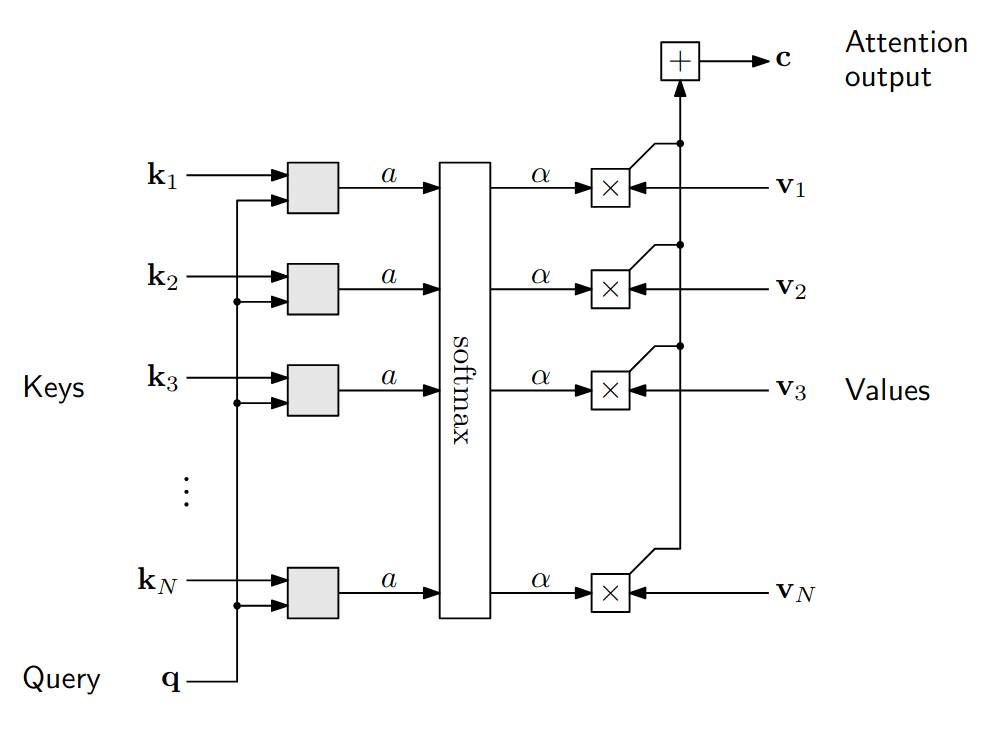
\includegraphics[width=0.7\linewidth]{figs/attnCompGraph}
	\caption{گراف محاسباتی بلوک توجه}
	\label{fig:attncompgraph}
\end{figure}


\textbf{تفسیر امتیاز توجه:}  
یکی از محدودیت‌های مهم در مدل‌های مبتنی بر بردار زمینه‌ای که پیش از ظهور مکانیزم توجه استفاده می‌شد، این بود که تمامی اطلاعات متن به یک بردار واحد فشرده می‌شد. این فشرده‌سازی باعث از دست رفتن بخشی از اطلاعات مهم، خصوصاً در دنباله‌های طولانی، می‌شد. مکانیزم خودتوجه این محدودیت را با تخصیص وزن‌های متفاوت به نشانه‌های مختلف برطرف کرد. به این ترتیب، هر نشانه می‌تواند  بدون نیاز به وابستگی به یک نقطه مرکزی، اطلاعات موردنیاز خود را به‌طور مستقیم از تمامی دیگر نشانه‌ها استخراج کند‍.

\textbf{تشابه به توجه در زندگی واقعی:}  
مکانیزم توجه شباهت زیادی به نحوه پردازش اطلاعات در ذهن انسان دارد و مستقیما از مدل ذهنی انسان الهام گرفته است. هنگامی که به یک پاراگراف از متن یا یک تصویر نگاه می‌کنیم، توجه ما به بخش‌های مختلف بسته به اهمیت آنها جلب می‌شود. برای مثال، هنگام خواندن یک جمله، ممکن است بر کلمات کلیدی تمرکز کنیم که برای درک معنای کلی ضروری هستند. مکانیزم توجه در شبکه‌های عصبی نیز به‌طور مشابه عمل می‌کند و وزن بیشتری به اطلاعات مرتبط‌تر اختصاص می‌دهد، در حالی که اطلاعات کم‌اهمیت‌تر را نادیده می‌گیرد. این فرآیند باعث بهبود کارایی مدل ها می‌شود؛ چرا که به مدل توانایی دسترسی با وزن دلخواه به هر بخشی از ورودی را می‌دهد.

\section{مکانیزم خودتوجه در معماری های کاهشی-افزایشی}
اگرچه مکانیزم خودتوجه اغلب به‌عنوان یکی از ویژگی‌های برجسته معماری‌های ترنسفورمر شناخته می‌شود، می‌توان آن را به معماری‌های بازگشتی نیز اضافه کرد تا محدودیت‌های آن‌ها در مدیریت وابستگی‌های بلندمدت کاهش یابد. ایده این است که به جای وابستگی صرف به حالات بازگشتی، رمزگذار و رمزگشا می‌توانند با استفاده از مکانیزم خود-توجه، ارتباطات مستقیم بین نشانه‌های ورودی یا خروجی را مدلسازی کنند.

در هنگام رمزگشایی‌، بجای استفاده از بردار واحد $c$ که می‌توانست موجب از دست رفتن اطلاعات شود،‌ برای هر گام زمانی $t$ یک بردار زمینه $c_t$ محاسبه می‌کنیم. این محاسبه بر پایه مکانیزم خودتوجه است؛ به این صورت که Value ها و Key ها همان وضعیت های نهان  \textbf{کدگذار} (${h_1, h_2, \dots, h_N}$ ) و Query مقدار فعلی حالت پنهان \textbf{کدگشا} است.  

کلیدها ($\mathbf{K}$): نمایانگر ویژگی‌های رمزگذاری‌شده توالی ورودی هستند که از حالات پنهان انکدر استخراج می‌شوند: 
$$
K = \{h_1, h_2, \dots, h_N\},
$$
که در آن $ h_n $​ حالت پنهان کدگشا در گام زمانی $\mathbf{n}$ است.

مقادیر ($\mathbf{V}$): شامل همان اطلاعات کلید ها هستند. در اصل مقادیر بردار هایی هستند که امتیاز $\alpha$ توجه بر آن ها اعمال شده و میانگین وزنی مقادیر است که بردار $c_t$ را می‌سازد.
$$
K = \{h_1, h_2, \dots, h_N\},
$$
که در آن $ h_n $​ حالت پنهان کدگشا در گام زمانی $\mathbf{n}$ است.


پرسش‌ها ($\mathbf{Q}$):
نمایانگر حالت پنهان فعلی دیکدر در گام زمانی  $t-1 $ هستند:  
$$
Q = s_{t-1},
$$
که در آن \( s_{t-1} \) حالت پنهان دیکدر در گام زمانی قبلی است.

امتیاز هم‌راستایی بین کوئری $Q$ و هر کلید $ K_n $  با استفاده از تابع امتیازدهی محاسبه می شود که قبلا توضیح داده شد.
$$
a_{t, n} = \text{score}(Q, K_n).
$$

سپس این امتیاز ها بیشینه‌نرم شده و وزن های توجه را می‌سازند.
$$
\alpha_{t, n} = \frac{\exp(a_{t, n})}{\sum_{n'=1}^N \exp(a_{t, n'})}.
$$

بردار زمینه  
بردار زمینه $ c_t $ در گام تولید $t$ به صورت ترکیب وزنی مقادیر $\mathbf{V}$
محاسبه می‌شود:  
$$
c_t = \sum_{n=1}^N \alpha_{t, n} h_n.
$$


 کدگشا مانند قبل بروزرسانی می‌شود.  
$$
s_t = g(y_{t-1}, c_t, s_{t-1}),
$$
که در آن $g$ معمولاً یک \lr{RNN}، یک
LSTM
 یا GRU است.

این مکانیزم به‌صورت پویا تعیین می‌کند که کدام توکن‌های ورودی برای گام فعلی دیکدر مهم‌تر هستند. این ویژگی نه تنها عملکرد بهتری بر روی توالی‌های بلند ارائه می‌دهد، بلکه با نمایش وزن‌های توجه $\alpha_{t,n}$ امکان تفسیر مدل را هم فراهم می‌کند و وابستگی مدل به یک بردار واحد را کم می‌کند. به وضوح این روش نیازمند محاسبات بیشتری است و از پیچیدگی زمانی بیشتری برخوردار است.

\section{مدل‌های ترنسفورمر}

مدل‌های ترنسفورمر که برای اولین بار در \cite{vaswaniAttentionAllYou2023} معرفی شدند، به‌طور کلی از معماری‌های جدیدی بهره می‌برند که از مکانیزم توجه به‌طور کامل استفاده می‌کنند. برخلاف مدل‌های سنتی seq2seq که از RNN یا LSTM برای پردازش توالی‌ها استفاده می‌کنند، ترنسفورمرها نیازی به پردازش ترتیبی ورودی‌ها ندارند و می‌توانند به‌طور همزمان کل توالی ورودی را پردازش کنند. این امر موجب می‌شود که مدل‌های ترنسفورمر برای پردازش داده‌های توالی بلند بسیار کارآمدتر از مدل‌های مبتنی بر RNN یا LSTM باشند.

در این بخش، به بررسی معماری ترنسفورمر و اجزای آن می‌پردازیم، از جمله مکانیزم توجه چندگانه، و معرفی مکانیزمی به نام جاسازی موقعیتی%
\LTRfootnote{Positional Embedding}
برای پردازش توالی‌های ورودی در مدلی که هدف آن موازی سازی است.
\subsection{مکانیزم توجه چندگانه \protect\LTRfootnote{Multi-Head Attention}}
در مدل‌های ترنسفورمر، توجه چندگانه به این صورت عمل می‌کند که چندین "سر توجه"%
\LTRfootnote{Attention Head}
به طور موازی اجرا می‌شوند. این امر به مدل این امکان را می‌دهد که از چندین نمایه مختلف از توالی ورودی برای محاسبه وزن‌های توجه استفاده کند.

فرایند توجه چندگانه به صورت زیر است:
\[
\text{MultiHead}(Q, K, V) = \text{Concat}(\text{head}_1, \dots, \text{head}_h) W^O
\]
که در آن:
\[
\text{head}_i = \text{Attention}(Q W_i^Q, K W_i^K, V W_i^V)
\]
در اینجا \( Q \)، \( K \)، و \( V \) به ترتیب کوئری‌ها، کلیدها و مقادیر هستند که از ورودی استخراج می‌شوند، و \( W_i^Q \)، \( W_i^K \)، و \( W_i^V \) ماتریس‌های وزن قابل یادگیری برای هر سر توجه هستند. \( W^O \) نیز ماتریس وزن نهایی است که پس از ترکیب تمام سرهای توجه، برای تولید نتیجه نهایی استفاده می‌شود.

در این معماری، به‌طور معمول از ۸ یا ۱۶ سر توجه استفاده می‌شود که به مدل این امکان را می‌دهد که توجه‌های مختلفی را در نقاط مختلف ورودی‌ها محاسبه کند و ویژگی‌های مختلفی از توالی‌ها را یاد بگیرد.

\subsection{جاسازی موقعیتی}

مدل‌های ترنسفورمر به طور ذاتی ترتیبی نیستند. این ویژگی یکی از عوامل اصلی موفقیت آنها محسوب می‌شود. در مقابل، مدل‌های بازگشتی مثل Seq2Seq به طور ذاتی ترتیبی هستند. این بدان معناست که پردازش ورودی‌ها در این مدل‌ها به صورت گام به گام انجام می‌شود و اطلاعات ورودی به صورت ترتیبی وارد مدل می‌شود. سؤال اصلی این است که چگونه می‌توان از این ویژگی ترتیبی مدل‌های RNN برای وظایف پردازش زبان استفاده کرد، هنگامی که معماری ما به یک معماری غیرترتیبی مثل ترنسفومر تغییر می‌یابد؟

تحقیقات نشان داد که می‌توان با استفاده از جاسازی موقعیتی، این مشکل را حل کرد. در این روش، برای مدل ترنسفورمر که به طور ذاتی ترتیبی نیست، اطلاعات موقعیتی به ورودی‌ها اضافه می‌شود. این امر به مدل این امکان را می‌دهد که ترتیب و موقعیت هر نشانه در توالی را در نظر بگیرد، بدون اینکه نیاز به پردازش ترتیبی ورودی‌ها باشد. به عبارت دیگر، \textbf{مدل‌های ترنسفورمر می‌توانند از طریق این جاسازی موقعیتی به صورت غیر ترتیبی عمل کنند، و در عین حال همچنان ویژگی‌های ترتیبی توالی‌ها را درک کنند}.

در این روش، به هر توکن ورودی یک بردار موقعیتی اضافه می‌شود تا اطلاعات مربوط به ترتیب آن در توالی به مدل منتقل شود. این بردارهای موقعیتی می‌توانند به‌طور دلخواه تولید شوند. Vaswani و همکاران در تحقیق خود چنین برداری را  به صورت زیر تعریف کرده اند:

\begin{equation}
PE(t, 2i) = \sin\left( \frac{t}{\lambda^{2i/d}} \right), \quad PE(t, 2i+1) = \cos\left( \frac{t}{\lambda^{2i/d}} \right)
\end{equation}
که در آن:
$t$ شماره توکن در توالی است،
$i$ شاخص بعد در بردار موقعیتی است،
و
$d$ ابعاد کل بردار موقعیتی است. 
همچنین $\lambda$ پیشنهاد شده توسط Vaswani و همکاران عدد ۱۰۰۰۰ (ده هزار) است که بسته به طول زمینه%
\LTRfootnote{Context Length}
مورد نظر در دنباله های ورودی، می‌تواند متغیر باشد.

این بردارهای موقعیتی به‌طور مستقیم به ورودی‌ها اضافه می‌شوند و به مدل این امکان را می‌دهند که ترتیب نشانه‌ها را در توالی در نظر بگیرد. این روش به‌ویژه در مواقعی که توالی‌ها طولانی هستند، اهمیت زیادی دارد، زیرا باعث می‌شود که مدل بتواند به راحتی به ترتیب نشانه‌ها نیز توجه کند.

\begin{figure}
	\centering
	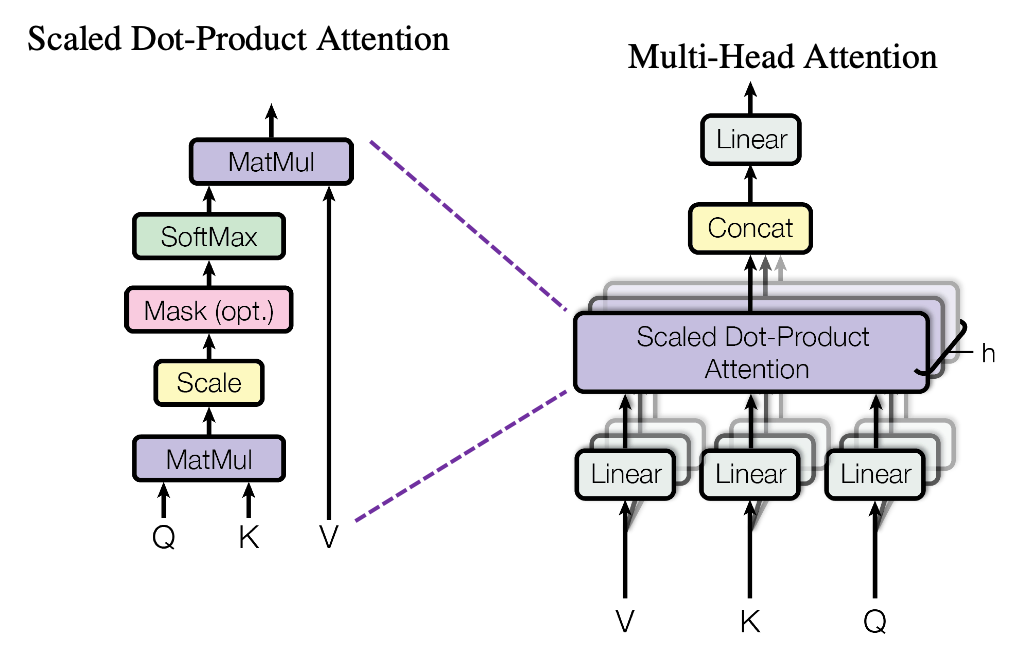
\includegraphics[width=0.7\linewidth]{figs/mhattn1.png}
	\caption{دیاگرام معماری توجه چندگانه}
	\label{fig:mhattn1}
\end{figure}


\subsection*{ساختار مدل ترنسفورمر}
مدل ترنسفورمر از دو بخش اصلی تشکیل شده است: رمزگذار و رمزگشا. هر یک از این بخش‌ها شامل چندین لایه هستند که هر کدام شامل مکانیزم‌های توجه چندگانه و یک شبکه عصبی کاملاً متصل (Feed-Forward Neural Network) هستند. در هر لایه، ابتدا توجه چندگانه اعمال می‌شود، سپس نتیجه با یک شبکه عصبی کاملاً متصل (FCN) پردازش می‌شود و در نهایت با استفاده از یک نرمال‌سازی و اعمال یک لایه کانولوشنی، نتیجه نهایی به‌دست می‌آید.


%
%\subsection*{معادلات ترنسفورمر}
%مدل ترنسفورمر به طور خلاصه شامل مراحل زیر است:
%
%1. **لایه توجه چندگانه**:
%\[
%\text{MultiHead}(Q, K, V) = \text{Concat}(\text{head}_1, \dots, \text{head}_h) W^O
%\]
%که هر سر توجه به صورت زیر عمل می‌کند:
%\[
%\text{head}_i = \text{Attention}(Q W_i^Q, K W_i^K, V W_i^V)
%\]
%
%2. **شبکه عصبی کاملاً متصل**:
%\[
%\text{FFN}(x) = \max(0, x W_1 + b_1) W_2 + b_2
%\]
%که در آن \( W_1 \)، \( W_2 \) ماتریس‌های وزن و \( b_1 \)، \( b_2 \) بایاس‌ها هستند.
%
%3. **ساختار انکدر**:
%هر لایه انکدر شامل یک لایه توجه چندگانه و یک شبکه عصبی کاملاً متصل است:
%\[
%\text{EncoderLayer}(x) = \text{FFN}(\text{MultiHeadAttention}(x))
%\]
%این لایه‌ها به‌طور متوالی برای پردازش ورودی‌ها تکرار می‌شوند.
%
%4. **ساختار دیکدر**:
%دیکدر نیز مشابه انکدر است، اما تفاوت اصلی آن این است که ابتدا از توجه ماسک‌شده برای جلوگیری از دسترسی به آینده استفاده می‌کند. معادله مربوط به دیکدر به صورت زیر است:
%\[
%\text{DecoderLayer}(x) = \text{FFN}(\text{MultiHeadAttention}(\text{Masked}(x), \text{EncoderOutput}))
%\]
%در اینجا \( \text{Masked}(x) \) به این معنا است که توجه به ورودی‌ها تنها به توکن‌های قبلی محدود می‌شود.

\subsection*{نتیجه‌گیری}
مدل‌های ترنسفورمر با استفاده از مکانیزم توجه، به‌ویژه توجه چندگانه و جاسازی موقعیتی، به‌طور موثری می‌توانند توالی‌ها را پردازش کنند بدون اینکه نیاز به پردازش ترتیبی ورودی‌ها باشد. این ویژگی‌ها موجب می‌شوند که ترنسفورمرها برای پردازش داده‌های طولانی و پیچیده بسیار مناسب باشند و در بسیاری از وظایف مختلف پردازش زبان طبیعی، از جمله ترجمه ماشینی و تولید متن، به موفقیت‌های چشمگیری دست یافته‌اند.


\section{ترنسفورمر ها در ترمیم تصویر}

خاصیت های مطرح شده و موفقیت شگرف مدل های ترنسفورمر
\cite{radfordLanguageModelsAre2019}
\cite{brownLanguageModelsAre2020}
\cite{openaiGPT4TechnicalReport2024}
در مدل سازی دنباله های متنی طولانی، بدون از دست رفتن وابستگی های بلندمدت، موجب جلب توجه محققان به کاربرد آن‌ها در کابرد های پردازش تصویر نیز شده است.
\cite{liuSwinTransformerHierarchical2021}


یکی از اولین مدل‌های مطرح در این زمینه، مدل ویت (ViT) 
\cite{dosovitskiyImageWorth16x162021}
است که تصویر ورودی را به قطعات کوچک (پچ‌ها) تقسیم کرده و از این قطعه‌ها به عنوان دنباله ورودی به مدل استفاده می‌کند. تصویر ورودی را به صورت $I \in \mathbb{R}^{H \times W \times C}$ در نظر بگیرید که $H$ و $W$ به ترتیب ارتفاع و عرض تصویر و $C$ تعداد کانال‌ها (مانند ۳ در تصاویر \lr{RGB}) است. برای پردازش تصویر، ابتدا آن را به $N$ قطعه (پچ) با ابعاد $P \times P$ تقسیم می‌کنیم، به‌طوری‌که تعداد کل پچ‌ها از رابطه زیر به دست می‌آید:
\[
N = \frac{HW}{P^2}
\]
هر پچ را به‌صورت $x_i \in \mathbb{R}^{P \times P \times C}$ نمایش می‌دهیم. سپس دنباله‌ای از این پچ‌ها به صورت زیر تعریف می‌شود:
\[
X_P = [x_1, x_2, \dots, x_N] \in \mathbb{R}^{N \times (P^2 \cdot C)}
\]
به‌منظور تبدیل این دنباله به فضای ویژگی‌های مدل، یک نگاشت خطی قابل آموزش $E \in \mathbb{R}^{P^2 \cdot C \times D}$ تعریف می‌شود که در آن $D$ بعد فضای جاسازی است.
\footnote{نمونه ای از اعداد مناسب برای این بعد ۱۲۸، ۵۱۲ یا ۱۰۲۴ است. بدیهی است ابعاد بیشتر ویژگی های بیشتری یاد گرفته ولی هزینه پردازش را به‌شدت افزایش می‌دهند.}
 نتیجه نگاشت خطی به صورت زیر خواهد بود:
\[
Z = X_P \cdot E
\]
که در آن $Z \in \mathbb{R}^{N \times D}$ دنباله جاسازی‌شده ورودی است. 

این ساختار، تصویر ورودی را به دنباله‌ای از بردارهای ویژگی تبدیل می‌کند که می‌توان آن را به مدل ترنسفورمر ارائه داد. ویژگی برجسته این روش، امکان مدل‌سازی وابستگی‌های بلندمدت بین قطعه های تصویر و ترکیب اطلاعات محلی و سراری است. این خصوصیت به‌ویژه در کاربردهایی نظیر ترمیم تصویر اهمیت دارد، چرا که در این مسائل، مدل نیازمند بازیابی نواحی آسیب‌دیده بر اساس نواحی مشاهده‌شده است.

در روش‌های ترمیم تصویر مبتنی بر ترنسفورمر، نواحی ماسک‌شده تصویر با پچ‌هایی مشخص می‌شوند که اطلاعات آن‌ها حذف شده است. سپس مدل ترنسفورمر با استفاده از دنباله جاسازی‌شده $Z$، ارتباطات بین پچ‌های مشاهده‌شده و ماسک‌شده را مدل‌سازی کرده و اقدام به بازسازی پچ‌های ماسک‌شده می‌کند. این رویکرد امکان ترمیم نواحی پیچیده تصویر با استفاده از اطلاعات زمینه‌ای را فراهم می‌سازد.



یکی از چالش های استفاده از این معماری در پردازش تصویر، هزینه هنگفت  استفاده از مکانیزم توجه مبتنی بر فضا (به معنی کار با داده های پیکسلی خام در فضا) است.

یکی از راه های مقابله با این چالش،‌ استفاده از نمونه‌برداری کاهشی برای کاهش وضوح تصویر (اما همچنان در فضای پیکسل) است. 


راه دیگر، این است که ابتدا تصاویر را به ویژگی های با وضوح پایین‌تر در یک فضای فشرده رمزگذاری کنیم.

اما 

